\documentclass[aps,prd,onecolumn,nofootinbib,superscriptaddress]{revtex4-2}

\usepackage[utf8]{inputenc}
\usepackage[T1]{fontenc}
\usepackage{lmodern}
\usepackage{amsmath,amssymb,amsfonts,bm}
\usepackage{graphicx}
\usepackage{xcolor}
\usepackage{hyperref}
\usepackage{siunitx}
\usepackage{enumitem}
\usepackage{booktabs}

\hypersetup{colorlinks=true,linkcolor=blue,citecolor=blue,urlcolor=blue}
\graphicspath{{../figs/}{TCV-PHI/papers/paper-09/figs/}}

\newcommand{\dd}{\mathrm{d}}
\newcommand{\trm}{\mathrm}
\newcommand{\qsp}{\ensuremath{Q_{\mathrm{SP}}}}

\begin{document}

\title{TCV-\texorpdfstring{$\phi$}{phi} IX: mesoscopic quasiparticle families from cohesive vacuum microstructure}

\author{Cyrille LECROQ}
\affiliation{Independent Researcher}

\date{\today}

\begin{abstract}
We present the first consolidated mesoscopic quasiparticle layer of the TCV-$\phi$ framework.
The analysis starts from the scale mismatch between a single CC-$\Phi_1$ cluster and an observed particle-like object and replaces the mono-cluster reading by localized coherent patch excitations.
At patch level, the composite observable \qsp emerges as the best current transport-level carrier of quasiparticle identity, with mean invariant retention $\simeq 0.94$ and mean identity score $\simeq 0.97$, outperforming the raw signed invariant.
Collision and recombination scans then collapse onto reduced attractor classes, from which we obtain a robust charge-like ladder, a stabilized spectral bridge with full order retention on the frozen basis, and a neutral five-slot observable basis consisting of a light recombined pair and a differentiated heavy transported triplet.
The resulting structure supports a controlled family-level rapprochement, while remaining explicitly below the threshold of exact Standard Model identification.
\end{abstract}

\maketitle

\section{Introduction}
The question addressed here is whether the TCV-$\phi$ microstructure supports a non-arbitrary particle-level effective organization once the identification ``one cluster = one particle'' is abandoned.
The answer emerging from the present scans is affirmative, but only at mesoscopic level.
The relevant effective objects are localized coherent patches of CC-$\Phi_1$ clusters, not isolated clusters.

This shift is not cosmetic.
At mono-cluster level, transport, charge-like discrimination, and family-level stability remain too fragile.
At patch level, the same programme becomes materially more coherent:
PMNS-like behavior improves, transport can be stabilized, collision outcomes close onto reduced attractors, and the resulting reduced basis admits both a charge-like ladder and a stable heavy/light ordering.
The local microstructural background used here extends the previous TCV-$\phi$ programme rather than replacing it, in particular the canonical EFT setup, the CC-$\Phi_1$ microstructural programme, the empirical confrontation layer, and the emergent $\Phi_2$ bridge developed earlier \cite{TCVPhiPaperI,TCVPhiPaperV,TCVPhiPaperVII,TCVPhiPaperVIII}.

The purpose of the paper is to freeze this mesoscopic layer as a standalone result.
The claim is not a Standard Model derivation.
The claim is that the TCV-$\phi$ microstructure supports a reproducible quasiparticle framework with internal hierarchy, transport identity, reduced collision algebra, and family-level structure.

\section{Scope and claim window}
The claim window of the present paper is intentionally limited.
We do \emph{not} claim:
\begin{itemize}
  \item an exact reconstruction of Standard Model gauge charges,
  \item an exact observed mass spectrum,
  \item a full spin-statistics reconstruction,
  \item or an exact one-to-one identification between quasiparticle branches and named particles.
\end{itemize}
Instead, we claim that the TCV-$\phi$ microstructure supports an internally coherent mesoscopic quasiparticle layer with:
\begin{itemize}
  \item a preferred patch-based effective description,
  \item a reproducible transport identity observable centered on \qsp,
  \item reduced collision/recombination attractors and channels,
  \item a robust internal charge-like ordering,
  \item a stabilized heavy/light spectral split,
  \item a neutral observable mapping,
  \item and a controlled family-level qualitative correspondence.
\end{itemize}

\section{From local clusters to mesoscopic patches}
The local CC-$\Phi_1$ cluster remains the fundamental microstructural building block.
However, the scale separation between the cluster scale and observed particle scales makes the mono-cluster picture too rigid to carry the full effective particle identity.
The working object of the present paper is therefore a mesoscopic patch excitation characterized by localization, coherence, and transport properties defined on a finite neighborhood of clusters.

The preferred static window lies in the mesoscopic regime rather than at either extreme of localization.
In the current implementation, the best compromise is reached for patch sizes around $n_{\rm clusters}\sim 11$--$15$, with the best transport behavior near $n_{\rm clusters}=13$.
This is not merely a numerical convenience.
It changes the interpretation of the particle problem itself: mass-like, charge-like, and family-like properties are more naturally read as collective observables of a coherent patch than as attributes of a single microscopic building block.

This reframing also stabilizes the comparison with earlier work.
The local cluster geometry remains physically meaningful as the microscopic support layer, especially for the twisted multi-ring logic inherited from the local programme, but the observed particle-like object is now treated as the transported collective pattern built on top of that support.

\begin{figure}[t]
  \centering
  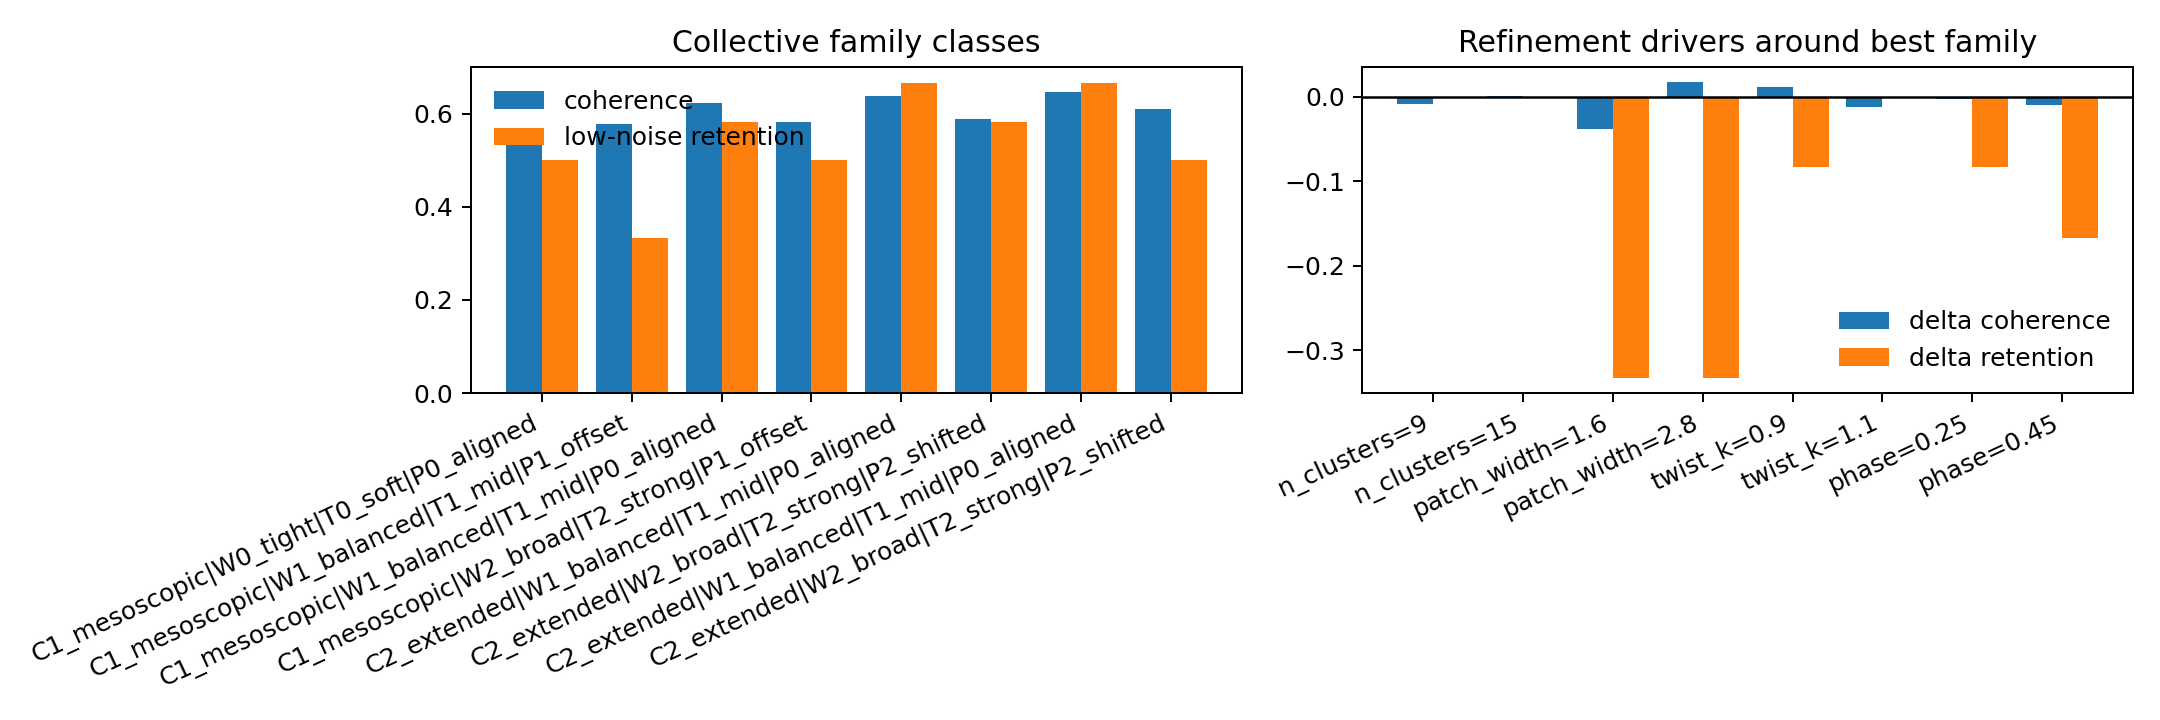
\includegraphics[width=0.88\textwidth]{paper-09-fig-01-mesoscopic-scale-hierarchy.png}
  \caption{Scale hierarchy and mesoscopic motivation for the patch-level quasiparticle picture. The effective particle carrier is treated as a coherent patch excitation rather than a mono-cluster object.}
  \label{fig:paper09-scale}
\end{figure}

\section{Transport identity and the role of \texorpdfstring{\qsp}{QSP}}
The first dynamical bottleneck of the patch framework is that the raw signed invariant is too fragile under transport.
The better dynamical carrier is the composite observable \qsp, which combines the signed content of the patch with a robust projection onto its canonical mesoscopic support branch.
Operationally, \qsp behaves as a transport-level identity coordinate: it preserves particle/antiparticle-like separation, remains compatible with the strongest propagation rules, and survives collisions and recombinations better than the raw signed invariant.

Quantitatively, the current transport scans give a mean \qsp\ retention near $0.94$ and a mean full identity score near $0.97$ for the best current composite candidate, while the raw signed invariant alone remains significantly more fragile.
The strongest rule in practice remains the relaxed transport rule.
By contrast, enforcing sign conservation alone improves the wrong quantity and degrades global identity retention.
The dynamical carrier is therefore composite rather than purely signed.

The present physical reading of \qsp\ is therefore precise but limited.
It should not yet be called an exact gauge charge.
The best interpretation is that of an effective transported identity observable with charge-like behavior under conjugation and collision.

\begin{figure}[t]
  \centering
  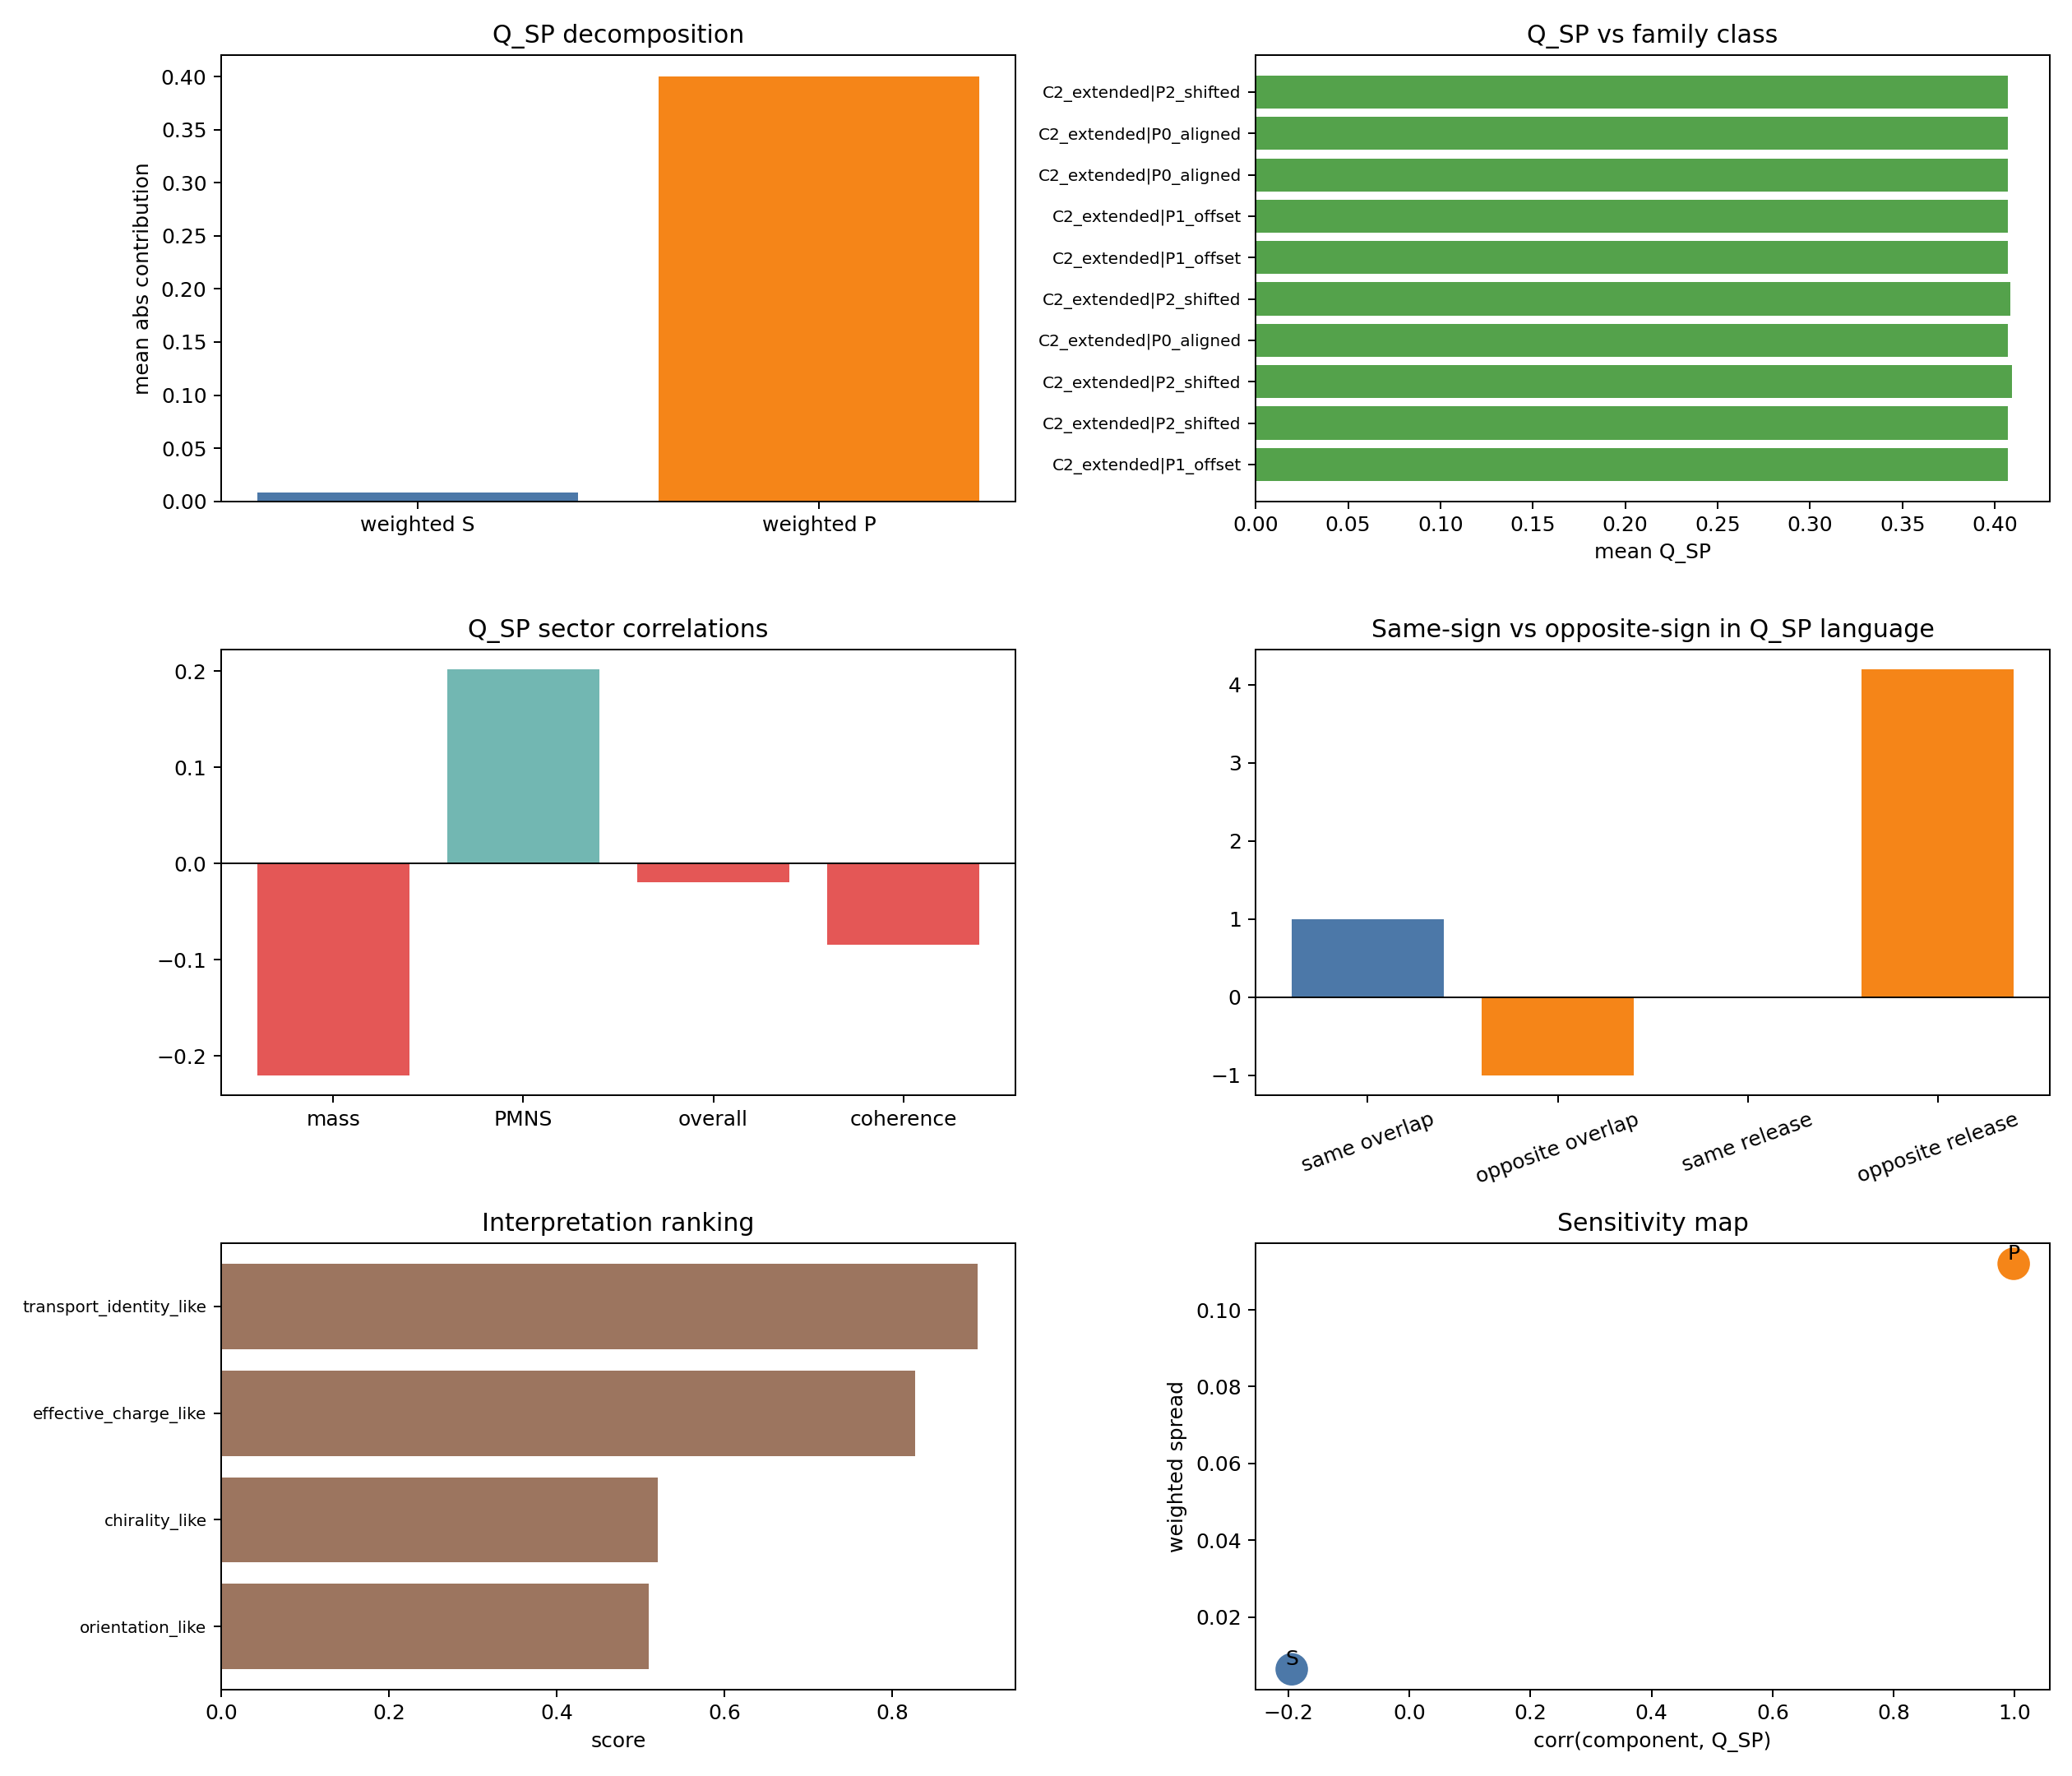
\includegraphics[width=0.92\textwidth]{paper-09-fig-02-qsp-identity-diagnostics.png}
  \caption{Diagnostics supporting the physical interpretation of \qsp as the best current transport-level quasiparticle identity observable.}
  \label{fig:paper09-qsp}
\end{figure}

\section{Collision channels, recombinations, and reduced attractors}
Once the quasiparticle identity is tracked by \qsp, patch collisions and recombinations can be classified in a non-arbitrary way.
The current programme exhibits several recurring channels, including coherent merges, asymmetric merges, residual recombinations, and annihilation-like endpoints.
These channels do not populate the final-state space uniformly.
Instead, they fall onto a reduced set of attractor classes.

This reduction is a structural result.
The mesoscopic dynamics is selective: only a limited subset of collective organizations remains dynamically favored after transport and interaction.
These attractors provide the basis for the effective family analysis developed later in the paper.

In the asymmetric collision scans, \qsp\ organizes the final channels much better than the raw signed invariant.
The cancellation proxy and the channel index both correlate much more strongly with total \qsp\ than with total signed content, showing that the collision problem is genuinely mesoscopic rather than just signed.
Once the attractors are reduced, a small number of classes dominate the post-collision population and become usable as effective building blocks for the next stages of the analysis.

\begin{figure}[t]
  \centering
  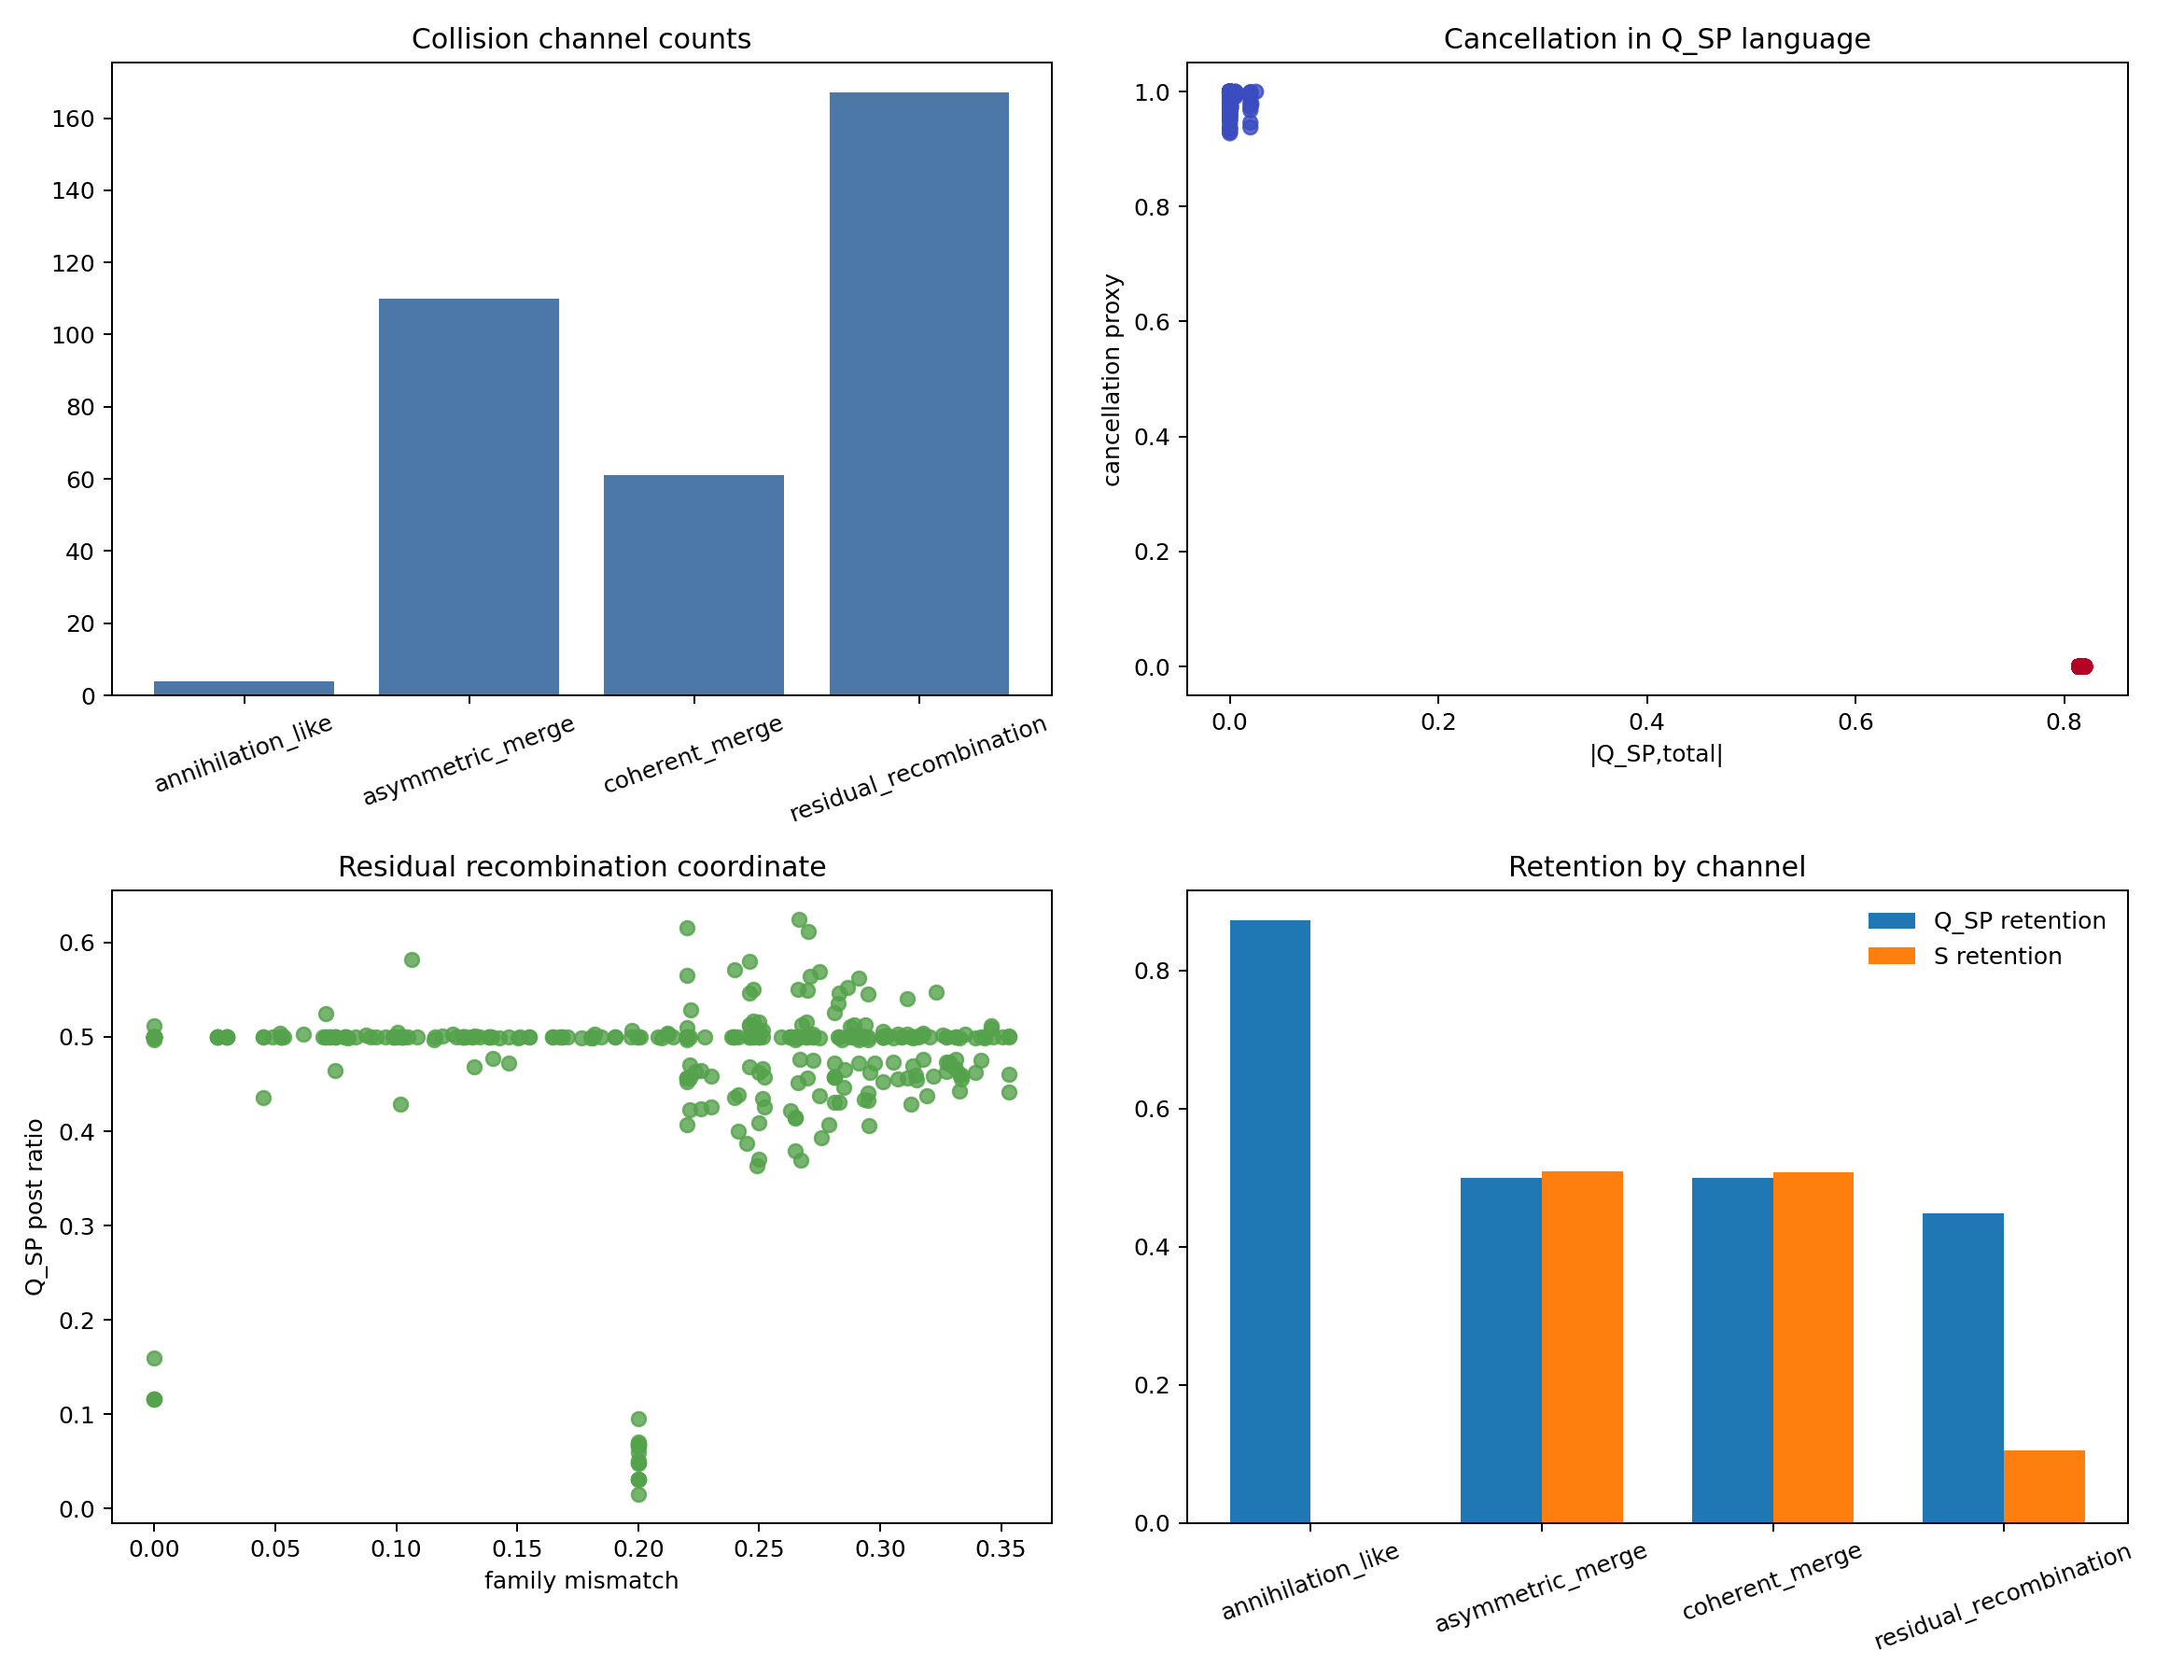
\includegraphics[width=0.92\textwidth]{paper-09-fig-03-collision-channels.png}
  \caption{Collision and recombination channels in the mesoscopic quasiparticle dynamics, organized in the \qsp-centered language.}
  \label{fig:paper09-collisions}
\end{figure}

\begin{figure}[t]
  \centering
  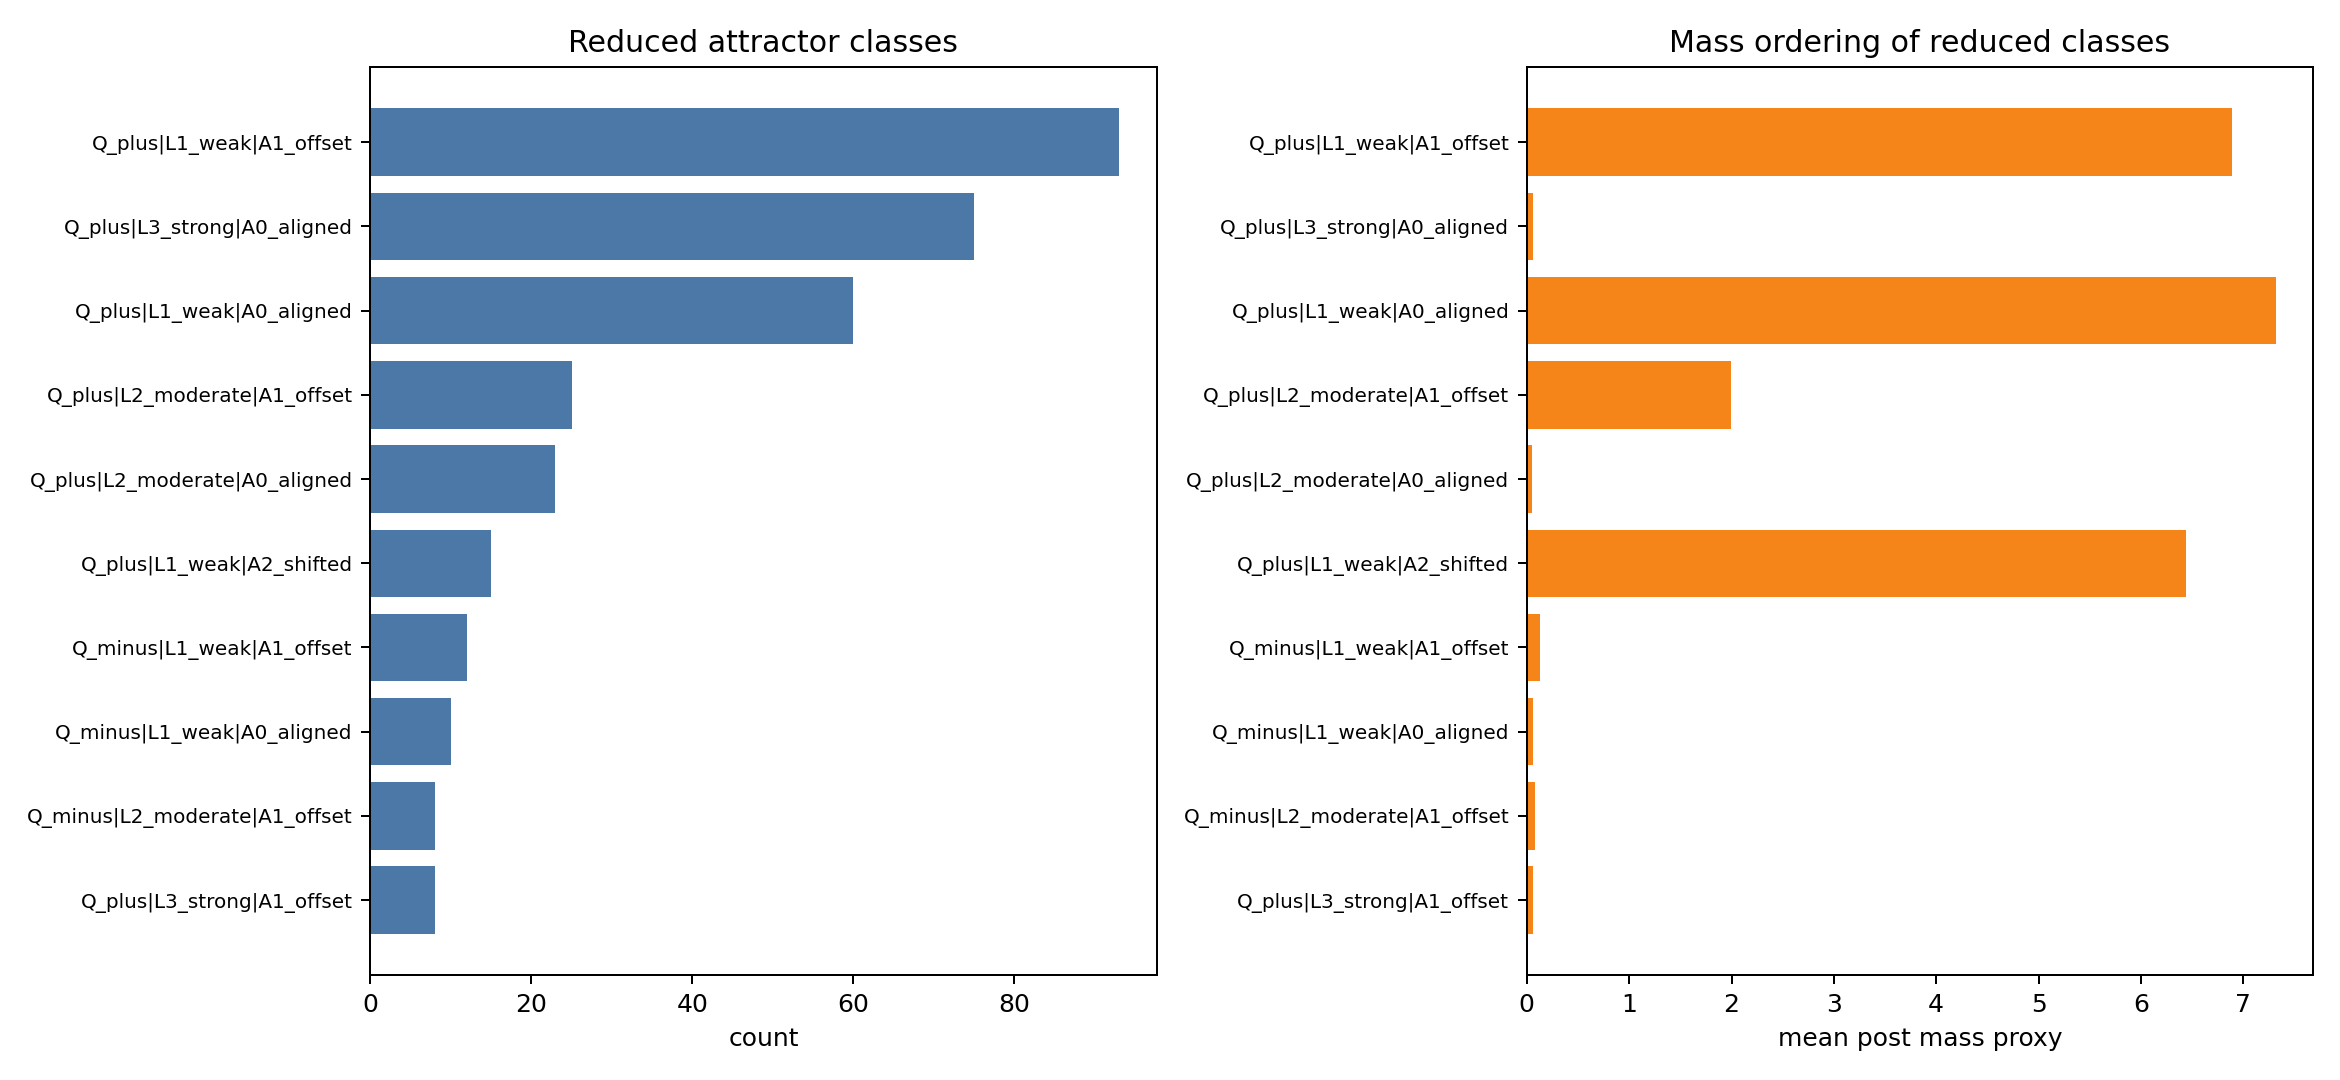
\includegraphics[width=0.84\textwidth]{paper-09-fig-04-attractor-reduction.png}
  \caption{Reduction of post-collision outcomes to a smaller set of mesoscopic attractor classes.}
  \label{fig:paper09-attractors}
\end{figure}

\section{Charge-like ladder and stabilized spectral bridge}
The reduced attractor classes admit a robust internal charge-like ordering once projected through the \qsp-based reconstruction and post-collision coherence support.
The resulting ladder separates positive heavy transported branches from negative light recombined branches while preserving internal structure inside each sector.
A separate spectral bridge, stabilized by combining mass proxy with transport robustness, yields a persistent heavy/light ordering that survives the tested perturbations.

The charge-like ladder is already more structured than a trivial $\pm$ split.
In the current frozen basis, the positive sector contains two strong positive states and one supported positive state, while the negative sector contains at least a weak and a moderate negative branch.
The sign separation survives the tested perturbations, and the level retention remains stable enough to justify a paper-level frozen ordering.

The spectrum bridge is now equally important.
The raw mass proxy alone was too fragile, but the stabilized bridge built from normalized post-collision mass proxy and transport robustness yields complete order retention on the frozen basis under the tested perturbations.
The heavy/light split is therefore no longer merely visual; it is a reproducible structural statement at the current toy level.

The key point is that the charge-like ladder and the spectral bridge are cross-compatible.
Their consistency yields the first robust internal observable map of the mesoscopic quasiparticle sector.

\begin{figure}[t]
  \centering
  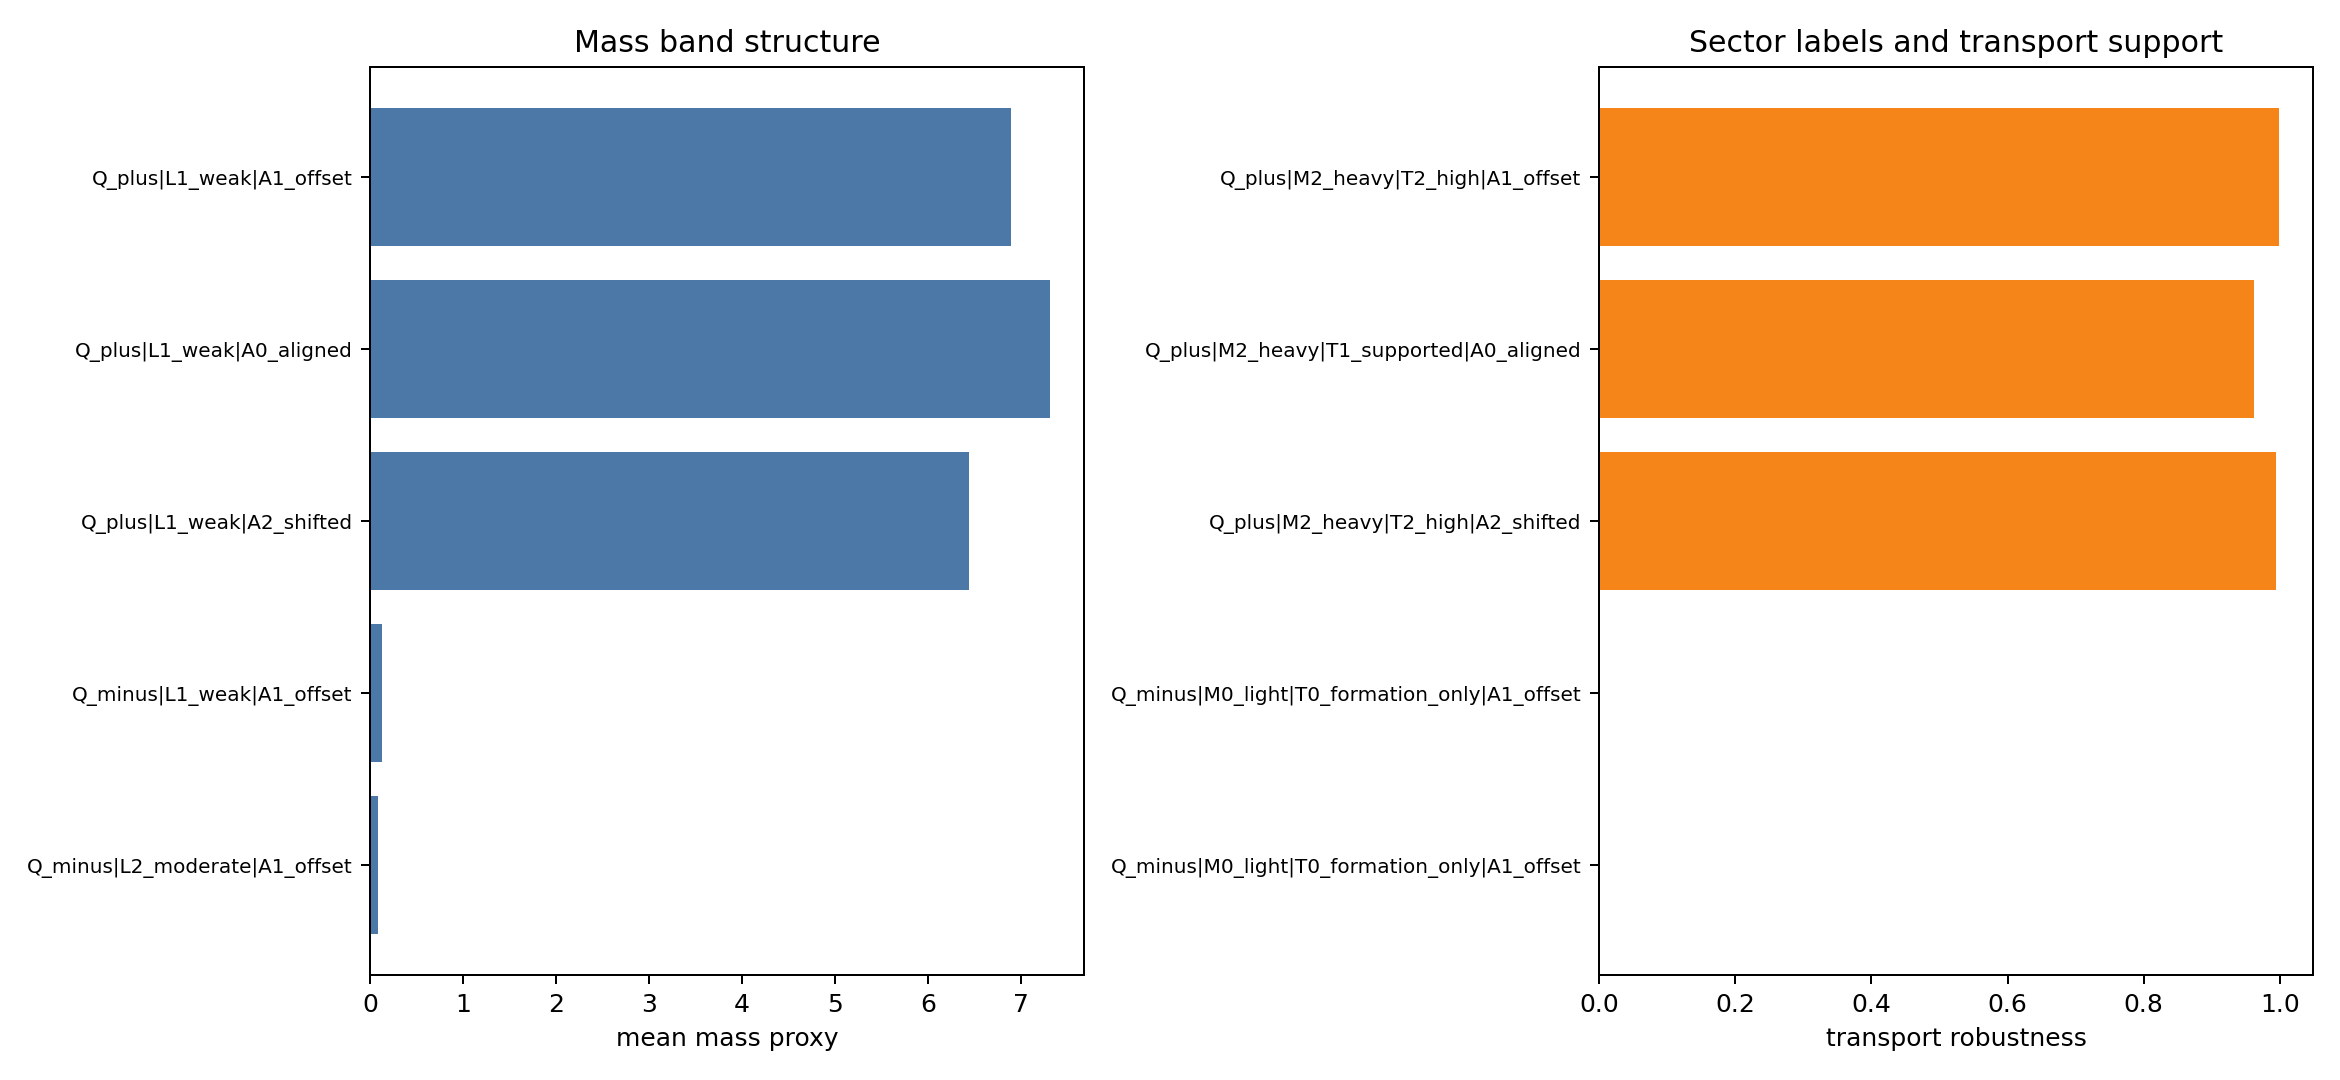
\includegraphics[width=0.92\textwidth]{paper-09-fig-05-sector-projection.png}
  \caption{Sector projection showing the stabilized heavy transported branches and the light recombined branches in the reduced quasiparticle basis.}
  \label{fig:paper09-sector}
\end{figure}

\section{Observable slots and effective family reading}
The stabilized cross structure defines a small set of neutral observable slots.
At the current stage, the reduced basis supports a low-rank light recombined pair and a differentiated heavy transported triplet.
These slots can be read as candidate effective families without assigning them named particle identities.
What matters is that the split is structurally supported by transport, collision, attractor, charge-like, and spectral diagnostics simultaneously.

\begin{table}[t]
  \centering
  \begin{tabular}{llll}
    \toprule
    Slot & Reduced class & Internal role & Effective reading \\
    \midrule
    OBS\_01 & $Q_{-}|L2|A1$ & negative recombination pole & light recombined pair \\
    OBS\_02 & $Q_{-}|L1|A1$ & negative recombination pole & light recombined pair \\
    OBS\_03 & $Q_{+}|L1|A2$ & shifted transport branch & heavy transported triplet \\
    OBS\_04 & $Q_{+}|L1|A1$ & offset transport branch & heavy transported triplet \\
    OBS\_05 & $Q_{+}|L1|A0$ & aligned transport branch & heavy transported triplet \\
    \bottomrule
  \end{tabular}
  \caption{Frozen neutral observable basis used in Paper IX. The notation is compressed: $Q_{\pm}$ denotes the sign sector, $Lk$ the reduced ladder level, and $Ak$ the reduced alignment branch.}
  \label{tab:paper09-observable-slots}
\end{table}

The current neutral observable basis contains five slots.
Two belong to a light recombined negative pair and three to a heavy transported positive triplet with shifted, offset, and aligned branches.
In internal shorthand, this yields a light paired family candidate and a heavy triplet family candidate.
The important point is not the labels themselves but that the split is non-arbitrary and reproduced by independent diagnostics.

At the same time, the two light slots remain dynamically weaker than the heavy transported branches.
In the current frozen basis they are formation-dominated states with vanishing mean transport robustness, so the light sector should presently be read as a recombination-supported sector rather than as a fully transported one.
This is a real limitation of the current programme and one of the clearest open problems left by the present paper.

This effective-family reading is therefore stronger than an analogy drawn by hand.
It emerges from the frozen chain:
patch picture $\rightarrow$ transport identity $\rightarrow$ collision channels $\rightarrow$ attractor reduction $\rightarrow$ charge-spectrum cross $\rightarrow$ neutral observable map.
That is why a family-level reading is now defensible even though exact particle naming remains blocked.

\begin{figure}[t]
  \centering
  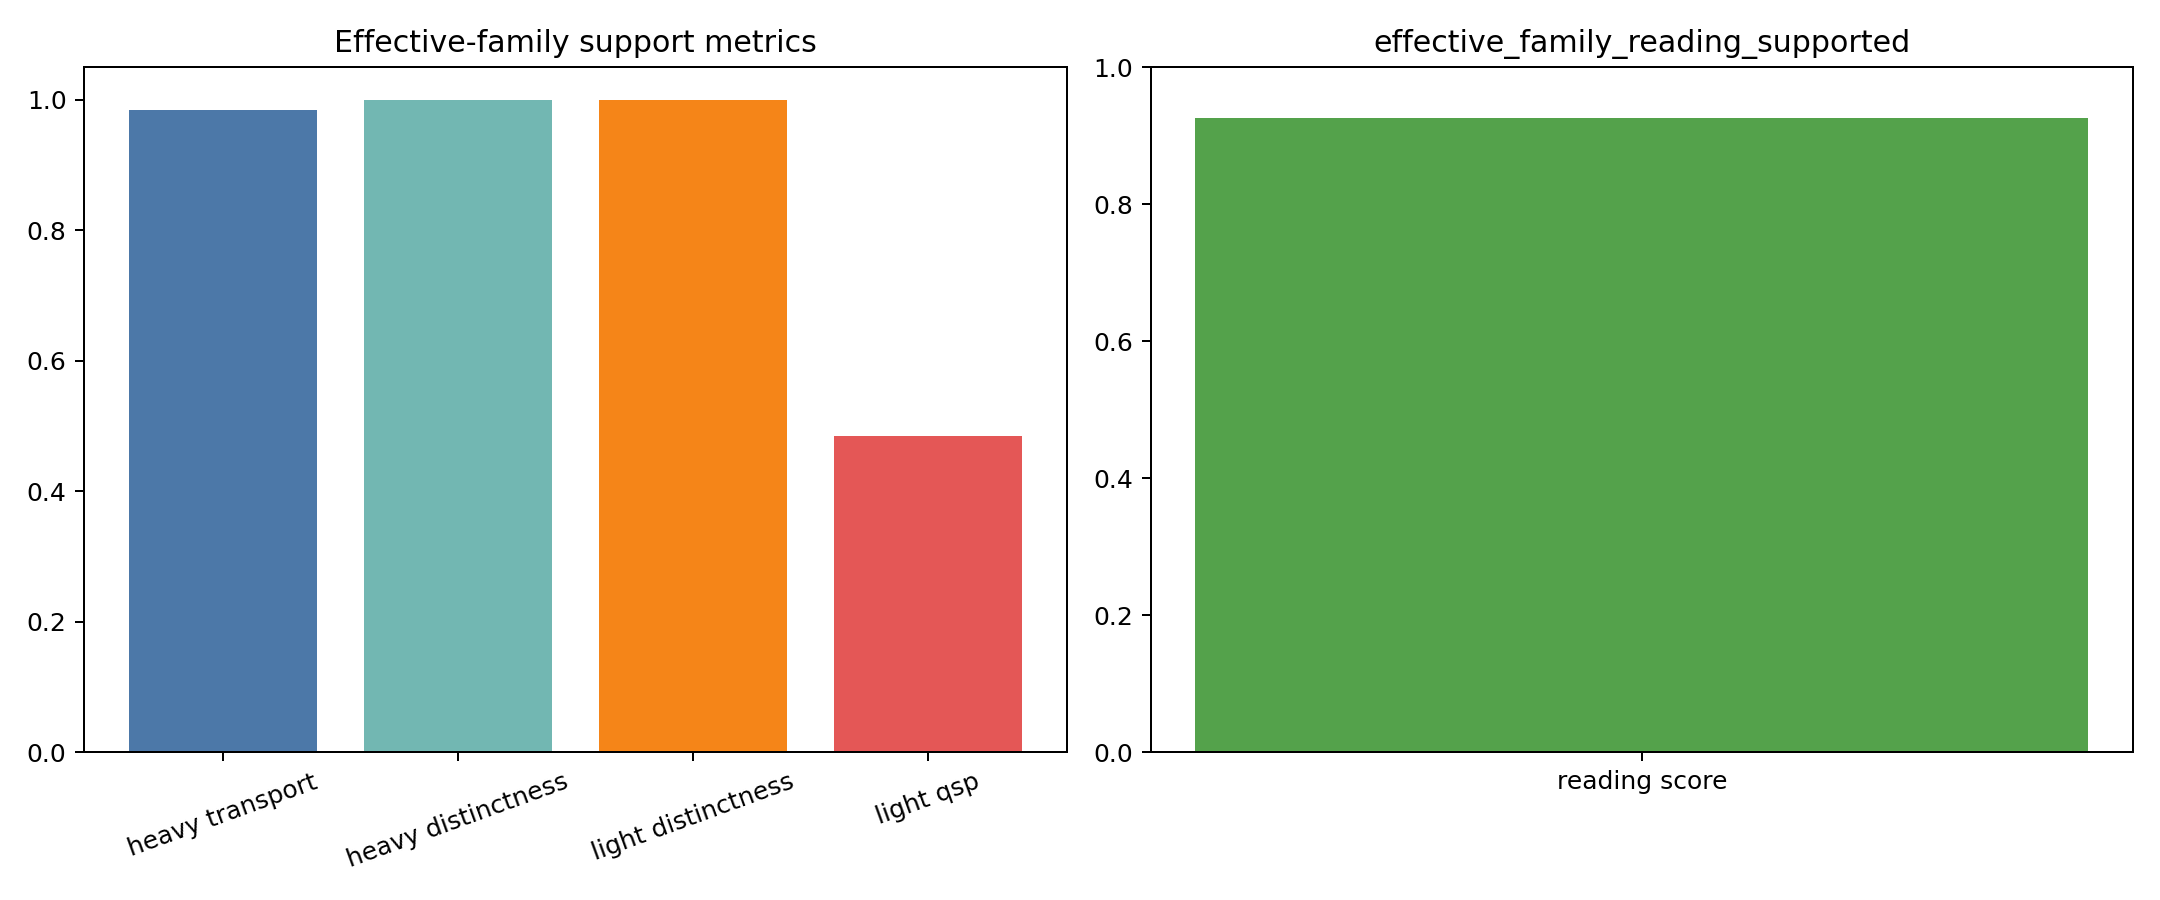
\includegraphics[width=0.88\textwidth]{paper-09-fig-06-effective-family-reading.png}
  \caption{Effective-family reading supported by the reduced quasiparticle basis: a light recombined pair and a differentiated heavy transported triplet.}
  \label{fig:paper09-family}
\end{figure}

\section{Controlled rapprochement and explicit limits}
The strongest interpretation allowed by the present evidence is a speculative but structured rapprochement with broad family-level particle organization.
The data support a heavy multibranch transported sector and a lighter recombined sector.
This is qualitatively compatible with a family-level reading, but several gates remain open before any exact mapping becomes defensible: exact charge reconstruction, spectroscopic calibration, spin/statistics closure, and explicit observable matching.

The rapprochement with broad Standard Model family patterns is therefore real but controlled.
The current evidence supports a light paired pattern and a heavier multibranch pattern with moderate internal confidence.
What remains explicitly blocked is exact identification:
the present framework does not yet reconstruct exact gauge charges, exact observed masses, or spin/statistics closure.

The present $2+3$ split also suggests a specific caution in interpretation.
Read literally, the reduced basis is closer to a paired light sector plus a triplet-like heavy sector than to a direct generation-by-generation replication of the full Standard Model spectrum.
If one attempts a qualitative rapprochement, the present structure therefore looks more naturally intragenerational than intergenerational.
This observation is only heuristic, but it is the appropriate way to read the current reduced basis.

This stopping point is deliberate.
The present result is already substantial without crossing that line.
It provides a disciplined bridge from cohesive-vacuum microstructure to a particle-like mesoscopic organization and freezes the first internally coherent family-level stage of the programme.

\section{Next gates}
The next technical gates are clear:
\begin{itemize}
  \item sharpen the charge-like reconstruction beyond the current internal ladder,
  \item calibrate the spectral bridge against stronger physical observables,
  \item incorporate spin/statistics information,
  \item and test whether the current family-level slots admit a tighter observable mapping.
\end{itemize}
These tasks belong to the next phase of the programme rather than to the claim window of the present paper.

\section{Conclusion}
The mesoscopic patch picture is now the best current effective particle-level description inside TCV-$\phi$.
Within this picture, \qsp\ emerges as the best current transport identity observable, collision-recombination dynamics closes onto reduced attractor classes, and the reduced basis supports both a robust charge-like ladder and a stabilized heavy/light spectrum bridge.
These structures in turn define a neutral observable basis and support a controlled effective-family reading.

The paper does not claim a full Standard Model derivation.
It does claim something narrower and stronger:
that the TCV-$\phi$ microstructure already supports a reproducible mesoscopic quasiparticle framework with internal hierarchy, transport identity, collision algebra, and family-level structure.
That is the result frozen here.

\begin{thebibliography}{5}

\bibitem{TCVPhiPaperI}
C.~Lecroq,
``TCV-$\phi$ I: an effective cohesive--vacuum field theory and its $\Lambda$CDM--compatible background cosmology,''
internal TCV-$\phi$ manuscript (2026).

\bibitem{TCVPhiPaperV}
C.~Lecroq,
``TCV-$\phi$ V: cohesive quantum microstructure from CC-$\Phi_1$ and a controlled bridge to CC-$\Phi_2$ flavour templates,''
internal TCV-$\phi$ manuscript (2026).

\bibitem{TCVPhiPaperVII}
C.~Lecroq,
``TCV-$\phi$ VII: empirical confrontation with Planck likelihoods,''
internal TCV-$\phi$ manuscript (2026).

\bibitem{TCVPhiPaperVIII}
C.~Lecroq,
``TCV-$\phi$ VIII: toward a one-scalar completion from cohesive-vacuum topology and coherent-sector $\Phi_2$ emergence,''
internal TCV-$\phi$ manuscript (2026).

\end{thebibliography}

\end{document}
